\chapter{The predictor/corrector integration scheme}

\section{Motivation}

Given an ordinary differential equation,
\begin{equation}
  \dv{x}{t} = f(t, x(t))
  \label{eq:ode}
\end{equation}
and some initial condition at $t_0$, we may compactly write the unknown function at any discrete time $t_i \equiv i\,\Delta t$ as
\begin{equation}
  \begin{aligned}
    x(t_i) & = x(t_{i-1}) + \int_{t_{i-1}}^{t_i} \dv{x}{t'} \dd{t'} \\
    &                 \equiv x(t_{i-1}) + \int_{t_{i-1}}^{t_i} f(t', x(t')) \dd{t'}
    \label{eq:ode step}
  \end{aligned}
\end{equation}
Numerical integration schemes advance a solution from $t_{i-1}$ to $t_i$ by approximating this integral, often as a weighted sum of the integrand evaluated at intelligently chosen points within the interval\footnote{Many numerical integrators use much more sophisticated methods than a weighted sum, but the idea of intelligently evaluating the integrand remains the same.}.
This process---particularly evaluating the integrand---becomes vastly more complicated through the introduction of retardation effects, effectively turning \cref{eq:ode} into
\begin{equation}
  \dv{x}{t} = f(t, x(t), x(t - \tau_1), x(t - \tau_2), \ldots).
  \label{eq:delay rhs}
\end{equation}
Causality imposed by the propagation operators only requires $\tau_j > 0$, thus \cref{eq:delay rhs} can relate a derivative to quantities arbitrarily far back in time, often between the discrete $t_i$/known solution values.
Further problems arise when $\tau_j < \Delta t$; in such cases, the unknown $x(t_i)$ depends on an unknown $x(t_i - \tau_j)$ which depends on an unknown $x(t_i - 2 \tau_j)$ etc., at least one of which lies ``ahead'' of the last known quantity, $x(t_{i-1})$.
While adjusting the timestep to require $t_j \geqslant \Delta t$ makes the system perfectly causal, it also makes the timestep prohibitively small for dense systems.
These constraints automatically exclude (or at least \emph{severely} limit the utility of) popular ODE algorithms and packages---the difficulty of reevaluating interactions prohibits variable-timestep integrators and integrators that require midpoint evaluations (such as the popular RK4 method) cannot accommodate small retardation factors without an exceptionally small $\Delta t$.
Instead, we turn to the exponentially-fitted predictor/corrector algorithm detailed in~\cite{}.
As a multistep method, the predictor/corrector does not require any function evaluations outside of those on the fixed timepoints, thus any causal interpolation scheme facillitates evaluating approximate versions of all the $x(t - \tau_j)$ via
\begin{equation}
  x(t_i - \tau_j) \approx \sum_{\ell = 0}^m w_\ell x\qty\big(t_i - (\floor{\tau_j/\Delta t} + \ell)\, \Delta t).
  \label{eq:interpolation}
\end{equation}
(The particular interpolation scheme determines the $w_\ell$.)
For $\tau_j < \Delta t$, \cref{eq:interpolation} suggests $x(t_i - \tau_j)$ becomes a function of $x(t_i)$.
Ordinarily, this would cause problems thought the predictor step of the algorithm ensures an approximate $x(t_i)$ exists before any interpolation.
The corrector step then works to correct this approximation in a convergent way, reincorporating adjacent sources as a total solution evolves.
  
\begin{figure}[]
  \centering
  \conditionalFigureInput{figures/time_circles.tex}
  \caption{\label{fig:retardation problem} Illustration of the ``retardation problem'' in solving coupled delay differential equations.
    The filled points indicate particle locations and the colored tangent lines mark the $x(t_i - \tau_j)$ quantities used in \cref{eq:interpolation}. 
    Because $\abs{\vb{r}_{\bullet \textcolor[RGB]{228,26,28}{\bullet}}} < c \, \Delta t$, determining $\qty{\vb{E}(\bullet, t),\vb{P}(\textcolor[RGB]{228,26,28}{\bullet}, t)}$ requires knowledge of $\qty{\vb{P}(\textcolor[RGB]{228,26,28}{\bullet}, t), \vb{E}(\bullet, t)}$.
  }
\end{figure}

\section{Integration coefficients}

\begin{figure}
  \centering
  \begin{subfigure}{0.4\textwidth}
    \centering
    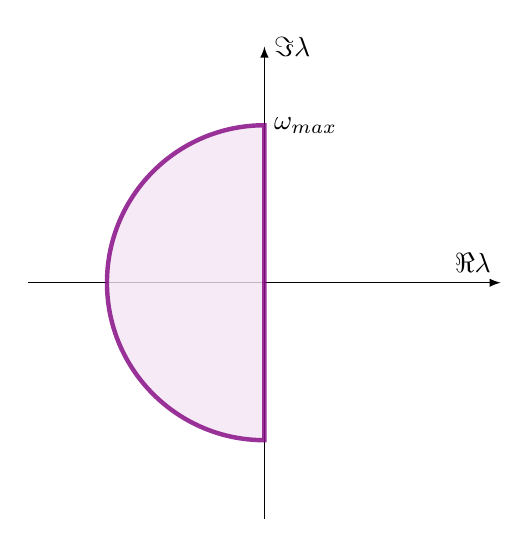
\begin{tikzpicture}[>=latex]
      \draw[->] (0,-3) -- (0, 3) node[right] {$\Im \lambda$};
      \draw[->] (-3,0) -- (3, 0) node[anchor=south east] {$\Re \lambda$};

      \draw[ultra thick, violet, fill=violet!10, opacity=0.8] (0,2) arc(-90:90:-2) -- (0,2) -- cycle;
      \node[right] at (0, 2) {$\omega_\text{max}$};
    \end{tikzpicture}
    \caption{\label{fig:filled semidisk}}
  \end{subfigure}
  \hspace{1cm}
  \begin{subfigure}{0.4\textwidth}
    \centering
    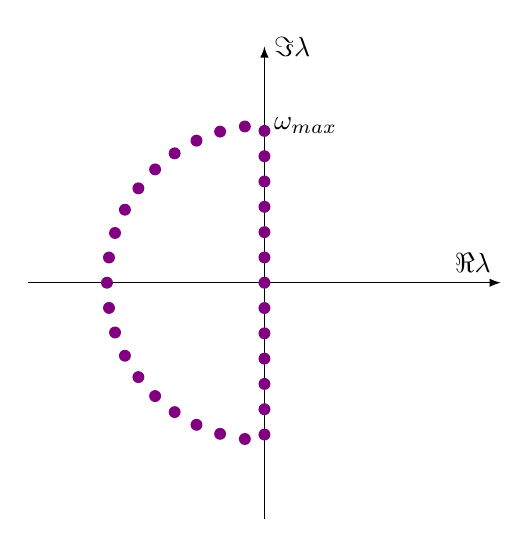
\begin{tikzpicture}[>=latex]
      \draw[->] (0,-3) -- (0, 3) node[right] {$\Im \lambda$};
      \draw[->] (-3,0) -- (3, 0) node[anchor=south east] {$\Re \lambda$};

      \foreach \point in {{0.,0.},{0.,0.32135},{0.,0.642699},{0.,0.964049},{0.,1.2854},{0.,1.60675},{0.,1.9281},{-0.248801,1.98446},{-0.563079,1.9191},{-0.862852,1.8043},{-1.1404,1.64301},{-1.38856,1.43941},{-1.60096,1.19872},{-1.77212,0.927148},{-1.89762,0.631695},{-1.97424,0.319969},{-2.,1.22465*10^-16},{-1.97424,-0.319969},{-1.89762,-0.631695},{-1.77212,-0.927148},{-1.60096,-1.19872},{-1.38856,-1.43941},{-1.1404,-1.64301},{-0.862852,-1.8043},{-0.563079,-1.9191},{-0.248801,-1.98446},{0.,-1.9281},{0.,-1.60675},{0.,-1.2854},{0.,-0.964049},{0.,-0.642699},{0.,-0.32135}}
      {
        \fill[violet] (\point) circle (0.5ex);
      }
      \node[right] at (0, 2) {$\omega_\text{max}$};
    \end{tikzpicture}
    \caption{\label{fig:discrete semidisk}}
  \end{subfigure}
  \caption{\label{fig:semidisk} Selection of the $\lambda_n$ parameters used in determining the predictor/corrector coefficients.
  }
\end{figure}

Let $x(t)$ denote the solution to a given ordinary differential equation.
We seek to approximate $x(t)$ as a linear combination of complex-valued exponentials such that
\begin{equation}
  x(t) \approx \sum_{\ell = 0}^{N_\lambda - 1} w_\ell e^{\lambda_\ell t}
  \label{eq:exponential approximation}
\end{equation}
for a given set of complex-valued $\lambda_\ell$ arguments and $w_\ell$ weights (never calculated explicitly).
As we wish to capture the behavior of physical systems---i.e.\ systems with exclusively oscillating and decaying modes---we choose the $\lambda_\ell$ to lie within the left half of the complex plane.
Moreover, assuming $x(t)$ contains little power above some threshold $\omega_\text{max}$, we select the $\lambda_\ell$ from within $S = \qty{z \in \mathbb{C} \, | \Re{z} \leqslant 0, \abs{z} \leqslant \omega_\text{max}}$: the left semidisk of radius $\omega_\text{max}$ (\cref{fig:filled semidisk}).
Finally, rather than choosing $\lambda_\ell$ from throughout $S$, the maximum modulus principle ensures that arguments taken from the boundary of $S$ in \cref{fig:discrete semidisk} will incur the maximum approximation error in \cref{eq:exponential approximation}. 
As a result, an approximation using $\lambda_\ell$ chosen from the boundary of $S$ accurately recovers the behavior of all modes with arguments in $S$.
In particular, we choose the $\lambda_\ell$ to have an equal spacing about the perimeter of $S$ (\cref{fig:discrete semidisk}).

If $x(t)$ and $\partial_t x(t)$ have known values at equidistant points $t_0, t_1, \ldots, t_{W - 1}$ on the interval $\qty[-1, 1]$ (thus $\Delta t = 2/(W - 1)$), we predict the value of $x(t_W)$ as a linear combination of past values and derivatives,
\begin{equation}
  x(t_W) \leftarrow \sum_{j = 0}^{W - 1} p_j x(t_j) + p_{j + W} \, \partial_t x(t_j).
  \label{eq:predictor}
\end{equation}
(The arrow here denotes an operation akin to assignment; this prediction does not \emph{define} $x(t_W)$, only the initial iteration of a process that will converge on $x(t_W)$.)
Inserting \cref{eq:exponential approximation} into this equation gives the matrix equation
\begin{equation}
  A \vb{p} = \vb{b}
  \label{eq:predictor vector}
\end{equation}
where
\begin{subequations}
\begin{align}
  A_{ij} &= \begin{cases}
    e^{\lambda_i t_j}, & 0 \leqslant i < N_\lambda; \; 0 \leqslant j < W \\
    \lambda_i e^{\lambda i t_{j - W}}, & 0 \leqslant i < N_\lambda; \; W \leqslant j < 2 W
  \end{cases} \label{eq:a matrix}\\
  b_i &= e^{\lambda_i t_W}. \label{eq:b vector}
\end{align}
\end{subequations}
Solving this equation for $\vb{p}$, then, produces the prediction coefficients in \cref{eq:predictor}.
Accordingly, we use a minimum-norm least-squares procedure to determine $\vb{p}$.
Having conjured an (approximate) value for $x(t_W)$, we may evaluate the prescribed ODE to obtain a value for $\partial_t x(t_W)$.
Writing
\begin{equation}
  x(t_W) \leftarrow \qty(\sum_{j = 0}^{W - 1} c_j x(t_j) + c_{W + j} \, \partial_t x(t_j)) + c_{2W} \, \partial_t x(t_W),
\end{equation}
this new equation reincorporates derivative information to refine the $x(t_W)$ approximation, requiring only a means of determining the $c_j$.
Again, inserting \cref{eq:exponential approximation} gives
\begin{equation}
  \tilde{A} \vb{c} = \vb{b}.
\end{equation}
Here,
\begin{equation}
  \tilde{A}_{ij} = \begin{cases}
    A_{ij}, & 0 \leqslant i < N_\lambda; \; 0 \leqslant j < 2W \\
    \lambda_i e^{\lambda_i t_W}, & 0 \leqslant i < N_\lambda; \; j = 2W
  \end{cases}
\end{equation}
$\vb{b}$ remains unchanged, and the same least-squares procedure determines $\vb{c}$.

Having derived the predictor/corrector coefficients for $h = 2/(W - 1)$---i.e.\ a uniform spacing between $W$ timepoints on the interval $\qty[-1, 1]$---the coefficients determined above require only a slight modification to accommodate systems with any $\Delta t$.
Noting that the formulation thusfar remains invariant under time translation and that the substitution $\tau = \alpha t$ (equivalently $\alpha = \Delta t/h$) turns
\begin{subequations}
\begin{equation}
  \pdv{\varphi(t)}{t} = \lambda \varphi(t)
\end{equation}
into
\begin{equation}
  \pdv{\varphi(\tau)}{\tau} = \frac{\lambda}{\alpha} \varphi(\tau),
\end{equation}
\end{subequations}
we need only scale the coefficients multiplying $\partial_t x(t_j)$ by $\alpha$ to adjust for other step sizes.
